\documentclass{article}

\usepackage{amsmath}
\usepackage{amssymb}
\usepackage{amsthm}
\usepackage{setspace}
\usepackage{graphicx}


\usepackage{amsmath,amsfonts}
\newtheorem{definition}{Definition}[section]
\newtheorem{fact}{Fact}[section]
\newtheorem{lemma}{Lemma}[section]
\newcommand{\eps}{\varepsilon}
\newcommand{\tab}{\hspace{.5cm}}
\newcommand{\R}{\mathbb R}
\newcommand{\N}{\mathcal N}
\newcommand{\norm}[1]{\left \lVert #1 \right \rVert}
\newcommand{\abs}[1]{\lvert #1 \rvert}
\newtheorem{theorem}{Theorem}[section]
\newtheorem{proposition}[theorem]{Proposition}
\newtheorem{corollary}[theorem]{Corollary}
\newtheorem{remark}[theorem]{Remark}

\title{Data mining: lecture 8} %
\author{Edo liberty, adapted from class notes by Yoel Shkolnisky}
\date{\nonumber}


\begin{document}

\maketitle

We will see that any
matrix $A \in \R^{m \times n}$ can be written as $A=U\Sigma V^{T}$ such that 
$U \in \mathbb{\R}^{m \times m}$ is unitary, $V \in \R^{n \times n}$ is unitary, and $\Sigma \in \mathbb{R}^{m
\times n}$ is a non-negative real diagonal matrix.
$\Sigma(i,i)$, denoted $\sigma_{i}$, are unique. If $A$ the singular values are distinct, then the singular vectors are
unique up to a multiplication by $z\in\mathbb{C}$ with $\abs{z}=1$.


\begin{remark}
Note the difference in notation from what we saw in class. 
The matrices $V$ and $U$ are what we denoted by $[V ; \overline{V}]$ 
and $[U ; \overline{U}]$ respectively. This makes the proofs a little cleaner
and hopefully more easy to follow. Note also that $\Sigma$ , unlike the matrix we denoted by $S$,
is not square. The non square matrix $\Sigma$ is still diagonal though, i.e. $\Sigma(i,j) = 0$ for all $i \ne j$. 
\end{remark}


\section{The geometry of SVD}
\begin{center}
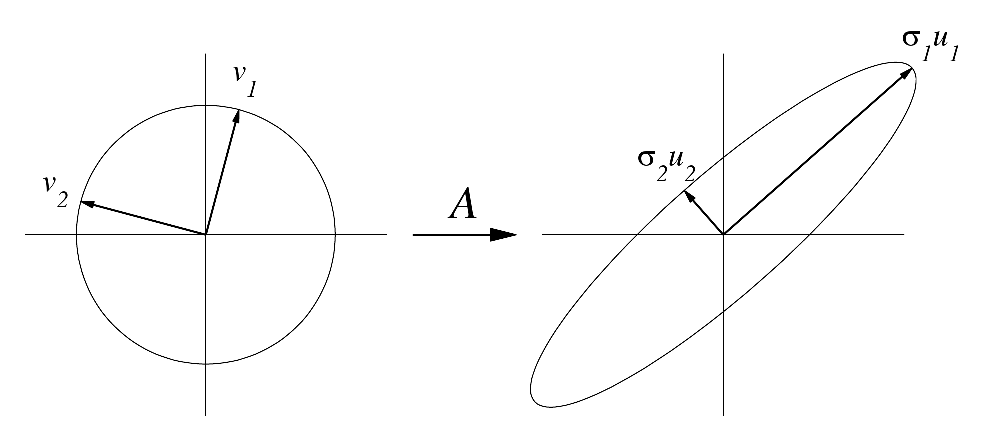
\includegraphics[width=0.6\textwidth]{images/SVDgeometry.eps}
\end{center}

\section{Proof of existence}
Set $\sigma_{1}=\norm{A}_{2}$. Let $u_{1}\in \mathbb{R}^{n}$ and
$v_{1}\in\mathbb{R}^{m}$ be unit 2-norm vectors such that $Av_{1} =
\sigma_{1}u_{1}$. To find these vectors, find the unit vector
$v_{1}$ that brings to maximum the expression
\begin{equation*}
\max_{\norm{x}=1} \norm{Ax}.
\end{equation*}
Then $A v_{1}=\mu u_{1}$ for some $\mu$ and a unit vector $u_{1}$.
Since $\norm{A v_{1}} = \sigma_{1}$, we get that $\sigma_{1} =
\norm{A v_{1}} = \abs{\mu} \norm{u_{1}} = \abs{\mu}$. Set $\mu =
\sigma_{1}$ to be positive, by flipping the sign of $u_{1}$ if
needed.

Complete $v_{1}$ into an orthonormal basis of $\mathbb{C}^{n}$,
denote $V_{1}$. Complete $u_{1}$ into an orthonormal basis of
$\mathbb{C}^{m}$, denoted $U_{1}$.
\begin{equation*}
S = U_{1}^{T} A V_{1}  = U_{1}^{T} \left [ \sigma_{1}u_{1} , A
v_{2}, \ldots, A v_{n}\right ] =
\begin{pmatrix}
\sigma_{1} & w^{T}  \\
0 & B
\end{pmatrix}.
\end{equation*}
We will show that $w^{T}=0$.
\begin{equation*}
\norm{S \begin{pmatrix} \sigma_{1} \\ w \end{pmatrix}}_{2} =  
\norm{
\begin{pmatrix}
\sigma_{1} & w^{T}  \\
0 & B
\end{pmatrix}
\begin{pmatrix}
\sigma_{1} \\ w
\end{pmatrix}
^{T}_{2}}
\ge \sigma_{1}^{2} + w^{T}w = \sqrt{\sigma_{1}^{2}+w^{T}w}
\norm{\begin{pmatrix} \sigma_{1} \\ w \end{pmatrix} }_{2}.
\end{equation*}
That is $\norm{S} \ge \sqrt{\sigma_{1}^{2} + w^{T}w}$. But
$\norm{S}_{2} = \norm{A}_{2}=\sigma_{1}$ and so $w=0$.

By induction, $B=U_{2}\Sigma_{2}V_{2}^{T}$ and
\begin{equation*}
A = U_{1}SV_{1}^{T} = U_{1}
\begin{pmatrix}
1 & 0 \\
0 & U_{2}
\end{pmatrix}
\begin{pmatrix}
\sigma_{1} & 0 \\
0 & \Sigma_{2}
\end{pmatrix}
\begin{pmatrix}
1 & 0 \\
0 & V_{2}^{T}
\end{pmatrix}
V_{1}^{T}.
\end{equation*}
The matrices
\begin{equation*}
U=U_{1}
\begin{pmatrix}
1 & 0 \\
0 & U_{2}
\end{pmatrix}, \quad
V=V_{1} \begin{pmatrix}
1 & 0 \\
0 & V_{2}^{T}
\end{pmatrix}
\end{equation*}
are unitary and the proof is complete.

\section{More properties of SVD}

% Is a matrix invertible, how far to singular, condition number, solving least squares. This SVD.

\begin{lemma}
The rank of $A$ equals the number of nonzero singular values.
\end{lemma}
\begin{proof}
Recall that if $B$ is $n \times k$ with rank $n$ than
$\operatorname{rank} (AB) = rank (A)$, and if $C$ is $l \times m$
with rank $m$ then $\operatorname{rank} (CA) = rank (A)$. Thus,
\begin{equation*}
\operatorname{rank} (A) = \operatorname{rank} (U \Sigma V^{T}) =
\operatorname{rank} (\Sigma V^{T}) = \operatorname{rank} (\Sigma).
\end{equation*}
Since $\Sigma$ is diagonal, its rank it the number its nonzero
elements.
\end{proof}

\begin{lemma}
Let $\operatorname{rank}(A)=r$.
Then,
\begin{align*}
\operatorname{range}(A) &= \operatorname{span}(u_{1},\ldots,u_{r}),\\
\operatorname{null}(A) &= \operatorname{span}(v_{r+1},\ldots,v_{n}).
\end{align*}
\end{lemma}

\begin{proof}
\begin{align*}
y \in \operatorname{range}(A) & \iff \exists x \text{ such that }
y=Ax \\
& \iff y=U\Sigma V^{T}x \\
& \iff y=U \Sigma z, \text{ where }z=V^{T}x \\
& \iff y = U \left (\sigma_{1} z_{1},\ldots,\sigma_r z_{r}, 0
,\ldots,0 \right )^{T} \\
& \iff y=\sum_{i=1}^{r} (\sigma_{i}z_{i}) u_{i} \\
& \iff y \in \operatorname{span} (u_{1},\ldots, u_{r}).
\end{align*}

\medskip

\begin{align*}
x \in \operatorname{null}(A) &\iff \norm{Ax}_{2}=0 \iff
\norm{U\Sigma V^{T} x}_{2}=0 \\
& \iff \norm{\Sigma V^{T}x}_{2} = 0 \iff \norm{\Sigma y}_{2} =0
\text{ where } y=V^{T}x \\
& \iff y=\left (0 ,\ldots,0,y_{r+1},\ldots,y_{n} \right
)^{T} \text{ where } y=V^{T}x\\
& \iff x=Vy,\ y=\left (0 ,\ldots,0,y_{r+1},\ldots,y_{n}
\right )^{T} \\
& \iff x=\sum_{i=r+1}^{n} y_{i} v_{i} \\
& \iff x \in \operatorname{span}(v_{r+1},\ldots,v_{n}).
\end{align*}

\end{proof}

\begin{lemma}
$\norm{A}_{2} = \sigma_{1}$ (even if you don't know the above
proof).
\end{lemma}
\begin{proof}
Immediate from the invariance of $\norm{\cdot}_{2}$ under unitary
transformations.
\end{proof}
Similarly, $\norm{A}_{F} = (\sigma_{1}^{2} + \cdots +
\sigma_{r}^{2})^{1/2}$.

\section{Relation between singular values and eigenvalues}
\begin{lemma}
The singular values of $A$ are the square roots of the nonzero
eigenvalues of $A^{T}A$ and $AA^{T}$.
\end{lemma}
\begin{proof}
If $A=U \Sigma V^{T}$, then $A^{T}=V \Sigma U^{T}$ and
\begin{equation*}
AA^{T} = \left (  U \Sigma V^{T} \right ) \left ( V \Sigma U^{T}
\right ) = U \Sigma \Sigma U^{T} = U \Sigma^{2} U^{-1}.
\end{equation*}
$AA^{T}$ is positive semi-definite and therefore all eigenvalues are
non-negative and there is no problem with the square root.
\end{proof}

Do not use this observation to compute the SVD! Reason: Assume for
simplicity that we have a $2 \times 2$ matrix $A$ (not diagonal)
whose SVD is given by $A = \sigma_{1} u_{1} v_{1}^{T} + \sigma_{2}
u_{2} v_{2}^{T}$ (See \ref{rank 1 approx} below). If
$\sigma_{2}/\sigma_{1} < 10^{-15}$, then the second term will
disappear due to round-off, that is, we cannot represent such a
matrix in double precision. Now, if the matrix $A$ has
$\sigma_{2}/\sigma_{1} < 10^{-8}$, then $A^{T}A$ and $AA^{T}$ have
ratio of singular values that is smaller than $10^{-15}$, and so
those matrices cannot be represented, and will be approximated as
rank-1 matrices with the second singular value being due to
round-off. In other words, although $A$ is not terribly conditioned,
we loose the small eigenvalues if we try to compute the SVD by
computing the eigenvalues of $A^{T}A$ or $AA^{T}$.

\begin{lemma}
If $A$ is hermitian, then the singular values of $A$ are the
absolute values of its eigenvalues.
\end{lemma}
\begin{proof}
A hermitian matrix is diagonalized by a unitary matrix with real
eigenvalues. That is,
\begin{equation*}
A=Q \Lambda Q^{T} = Q \abs{\Lambda} \operatorname{sign}(\Lambda)
Q^{T}.
\end{equation*}
Now set $U=Q$, $\Sigma=\abs{\Lambda}$,
$V^{T}=\operatorname{sign}(\Lambda) Q^{T}$.
\end{proof}

%%%\begin{lemma}
%%%The singular values of a matrix $A$ are precisely the lengths of the
%%%semi-axes of the ellipsoid defined by $E=\left \{ Ax \ : \
%%%\norm{x}_{2}=1 \right \}$.
%%%\end{lemma}

\section{Approximation properties}

\subsection{Rank-k approximation in the spectral norm}

\begin{lemma}\label{rank 1 approx}
$A$ can be written as a sum of rank-1 matrices. Explicitly,
\begin{equation*}
A = \sum_{j=1}^{r} \sigma_{j} u_{j} v_{j}^{T}.
\end{equation*}
\end{lemma}

\begin{theorem}
Set
\begin{equation*}
A_{k} = \sum_{j=1}^{k} \sigma_{j} u_{j} v_{j}^{T}.
\end{equation*}
Then,
\begin{equation*}
\min_{\substack{B \in \mathbb{C}^{m \times n} \\
\operatorname{rank}(B) \leq k}} \norm{A-B}_{2} = \norm{A-A_{k}}_{2}
= \sigma_{k+1}.
\end{equation*}
\end{theorem}
\begin{proof}
\begin{equation*}
A-A_{k} = \sum_{j=1}^{r} \sigma_{j} u_{j} v_{j}^{T} - \sum_{j=1}^{k}
\sigma_{j} u_{j} v_{j}^{T} = \sum_{j=k+1}^{r} \sigma_{j} u_{j}
v_{j}^{T}
\end{equation*}
and thus $\sigma_{k+1}$ is the largest singular value of $A-A_{k}$.
Alternatively, look at $U^{T} A_{k} V =
\operatorname{diag}(\sigma_{1},\ldots,\sigma_{k},0,\ldots,0)$, which
means that $\operatorname{rank}(A_{k}) = k$, and that
\begin{equation*}
\norm{A-A_{k}}_{2} = \norm{U^{T} (A-A_{k}) V}_{2} =
\norm{\operatorname{diag}(0,\ldots,0,\sigma_{k+1},\ldots,\sigma_{r})}_{2}
= \sigma_{k+1}.
\end{equation*}

Let $B$ be an arbitrary matrix with $\operatorname{rank}(B_{k}) =
k$. Then, it has a null space of dimension $n-k$, that is,
\begin{equation*}
\operatorname{null}(B) = \operatorname{span}(w_{1},\ldots,w_{n-k}).
\end{equation*}
A dimension argument shows that
\begin{equation*}
\operatorname{span}(w_{1},\ldots,w_{n-k}) \cap
\operatorname{span}(v_{1},\ldots,v_{k+1}) \ne \{ 0 \}.
\end{equation*}
Let $w$ be a unit vector from the intersection. Since
\begin{equation*}
Aw = \sum_{j=1}^{k+1} \sigma_{j} (v_{j}^{T}w) u_{j},
\end{equation*}
we have
\begin{equation*}
\norm{A-B}_{2}^{2} \ge \norm{(A-B)w}_{2}^{2} = \norm{Aw}_{2}^{2} =
\sum_{j=1}^{k+1} \sigma_{j}^{2} \abs{v_{j}^{T}w}^{2} \ge
\sigma_{k+1}^{2} \sum_{j=1}^{k+1} \abs{v_{j}^{T}w}^{2} =
\sigma_{k+1}^{2},
\end{equation*}
since $w \in \operatorname{span}\{v_{1},\ldots,v_{n+1}\}$, and the
$v_{j}$ are orthogonal.
\end{proof}

\subsection{Rank-k approximation in the Frobenius norm}

The same theorem holds with the Frobenius norm.
\begin{theorem} Set
\begin{equation*}
A_{k} = \sum_{j=1}^{k} \sigma_{j} u_{j} v_{j}^{T}.
\end{equation*}
Then,
\begin{equation*}
\min_{\substack{B \in \mathbb{C}^{m \times n} \\
\operatorname{rank}(B) \leq k}} \norm{A-B}_{F} = \norm{A-A_{k}}_{F}
= \sqrt{\sum_{i=k+1}^{n} \sigma_{i}^{2}}.
\end{equation*}
\end{theorem}
\begin{proof}
Suppose $A=U \Sigma V^{T}$. Then
\begin{equation*}
\min_{\operatorname{rank}(B) \leq k} \norm{A-B}^{2}_{F} =
\min_{\operatorname{rank}(B) \leq k} \norm{U \Sigma V^{T} - UU^{T} B
VV^{T}}^{2}_{F} = \min_{\operatorname{rank}(B) \leq k} \norm{\Sigma
- U^{T} B V}^{2}_{F}.
\end{equation*}
Now,
\begin{equation*}
\norm{\Sigma - U^{T} B V}^{2}_{F} = \sum_{i=1}^{n} \left (
\Sigma_{ii} - \left (U^{T}B V)_{ii} \right ) \right )^{2} +
\text{off-diagonal terms}.
\end{equation*}
If $B$ is the best approximation matrix and $U^{T}B V$ is not
diagonal, then write $U^{T}B V=D+O$, where $D$ is diagonal and $O$
contains the off-diagonal elements. Then the matrix $B = U D V^{T}$
is a better approximation, which is a contradiction.

Thus, $U^{T}B V$ must be diagonal. Hence,
\begin{equation*}
\norm{\Sigma - D}^{2}_{F} = \sum_{i=1}^{n} \left (\sigma_{i} - d_{i}
\right )^{2} = \sum_{i=1}^{k} \left (\sigma_{i} - d_{i} \right )^{2}
+ \sum_{i=k+1}^{n} \sigma_{i}^{2},
\end{equation*}
and this is minimal when $d_{i}=\sigma_{i}$, $i=1,\ldots,k$. The
best approximating matrix is $A_{k} = U D V^{T}$, and the
approximation error is $\sqrt{\sum_{i=k+1}^{n} \sigma_{i}^{2}}$.
\end{proof}


\subsection{Closest orthogonal matrix}
The SVD also allows to find the orthogonal matrix that is closest to
a given matrix. Again, suppose that $A = U \Sigma V^{T}$ and $W$ is
an orthogonal matrix that minimizes $\norm{A-W}^{2}_{F}$ among all
orthogonal matrices. Now,
\begin{equation*}
\norm{U \Sigma V^{T} - W}_{F}^{2} = \norm{U \Sigma V^{T} - UU^{T} W
VV^{T}} = \norm{\Sigma - \tilde{W}},
\end{equation*}
where $\tilde{W}=U^{T} W V$ is another orthogonal matrix. We need to
find the orthogonal matrix $\tilde{W}$ that is closest to $\Sigma$.
Alternatively, we need to minimize $\norm{\tilde{W}^{T} \Sigma -
I}_{F}^{2}$.

If $U$ is orthogonal and $D$ is diagonal and positive, then
\begin{equation}\label{eq1}
\begin{aligned}
\operatorname{trace} (UD) &= \sum_{i,k} u_{ik} d_{ki} \leq \sum _{i}
\left ( \left ( \sum_{k} u_{ik}^{2} \right )^{1/2} \left ( \sum_{k}
d_{ik}^{2} \right )^{1/2} \right ) \\
&= \sum_{i} \left ( \sum_{k} d_{ki}^{2} \right )^{1/2} = \sum_{i}
\left ( d_{ii}^{2} \right )^{1/2} = \sum_{i} d_{ii} =
\operatorname{trace}(D).
\end{aligned}
\end{equation}
Now
\begin{align*}
\norm{\tilde{W}^{T} \Sigma - I}_{F}^{2} &= \operatorname{trace}
\left ( \left( \tilde{W}^{T} \Sigma - I \right ) \left(
\tilde{W}^{T} \Sigma - I \right )^{T} \right ) \\
&= \operatorname{trace} \left ( \left( \tilde{W}^{T} \Sigma   - I
\right
) \left( \Sigma \tilde{W}  - I \right ) \right ) \\
&= \operatorname{trace} \left ( \tilde{W}^{T} \Sigma^{2} \tilde{W}
\right ) - \operatorname{trace} \left ( \tilde{W}^{T} \Sigma \right
) - \operatorname{trace} \left ( \Sigma \tilde{W} \right ) + n \\
&= \operatorname{trace} \left ( \left ( \Sigma \tilde{W} \right
)^{T} \left ( \Sigma \tilde{W}  \right ) \right ) - 2
\operatorname{trace} \left (\Sigma \tilde{W} \right ) + n \\
&= \norm{\Sigma \tilde{W}}_{F}^{2} - 2 \operatorname{trace} \left
(\Sigma \tilde{W} \right ) + n \\
&= \norm{\Sigma }_{F}^{2} - 2 \operatorname{trace} \left (\Sigma
\tilde{W} \right ) + n.
\end{align*}
Thus, we need to maximize $\operatorname{trace} \left (\Sigma
\tilde{W} \right )$. But this is maximized by $ \tilde{W} = I$ by
\eqref{eq1}. Thus, the best approximating matrix is $W=UV^{T}$.


\section{The ``Thin'' SVD}
Also called ``economy size'' SVD.  If $A \in \mathbb{C}^{m \times
n}$, $A=U \Sigma V^{T}$, and $m \ge n$, then the ``thin'' SVD is
$A=U_{1} \Sigma_{1} V^{T}$ where
\begin{equation*}
U_{1} = [u_{1},\ldots,u_{n}] \in \mathbb{C}^{m \times n}
\end{equation*}
and
\begin{equation*}
\Sigma_{1} = \operatorname{diag}(\sigma_{1},\ldots,\sigma_{n}) \in
\mathbb{R}^{n \times n}.
\end{equation*}


\section{Applications of the SVD}
\begin{enumerate}
\item Determining range, null space and rank (also numerical rank).
\item Matrix approximation.
\item Inverse and Pseudo-inverse: If $A=U \Sigma V^{T}$ and $\Sigma$
is full rank, then $A^{-1}=V \Sigma^{-1} U^{T}$. If $\Sigma$ is
singular, then its pseudo-inverse is given by $A^{\dagger}=V
\Sigma^{\dagger} U^{T}$, where $\Sigma^{\dagger}$ is formed by
replacing every nonzero entry by its reciprocal.
\item Least squares: If we need to solve $Ax=b$ in the least-squares
sense, then $x_{LS}=V \Sigma^{\dagger} U^{T} b$.
\item Denoising -- Small singular values typically correspond to
noise. Take the matrix whose columns are the signals, compute SVD,
zero small singular values, and reconstruct.
\item Compression -- We have signals as the columns of the matrix
$S$, that is, the $i$ signal is given by
\begin{equation*}
S_{i} = \sum_{i=1}^{r} \left ( \sigma_{j} v_{ij} \right ) u_{j}.
\end{equation*}
If some of the $\sigma_{i}$ are small, we can discard them with
small error, thus obtaining a compressed representation of each
signal. We have to keep the coefficients $\sigma_{j} v_{ij}$ for
each signal and the dictionary, that is, the vectors $u_{i}$ that
correspond to the retained coefficients.
\end{enumerate}


\section{Differences between SVD and eigen-decomposition}
\begin{enumerate}
\item Not every matrix has an eigen-decomposition (not even any
square matrix).  Any matrix (even rectangular) has an SVD.
\item In eigen-decomposition $A=X \Lambda X^{-1}$, that is, the
eigen-basis is not always orthogonal. The basis of singular vectors
is always orthogonal.
\item In SVD we have two singular-bases (right and left).
\item SVD tells everything on a matrix.
\item SVD as no numerical problems.
\item Relation to condition number; the numerical problems with
eigen-decomposition; multiplication by an orthogonal matrix is
perfectly conditioned.
\end{enumerate}


\section{Linear regression in the least-squared loss}
In Linear regression we aim to find the best linear approximation 
to a set of observed data. For the $m$ data  points $\{x_1,\ldots,x_m\}$,  $x_i \in \R^n$,
each receiving the value $y_i$, we look for the weight vector $w$ that minimizes:
\[
\sum_{i=1}^{n} (x_{i}^{T}w - y_i)^2 = \norm{Aw - y}_{2}^{2}
\]
Where $A$ is a matrix that holds the data points as rows $A_i = x^{T}_{i}$.

\begin{proposition}
The vector $w$ that minimizes $\norm{Aw - y}_{2}^{2}$ is $w = A^{\dagger}y = V\Sigma^{\dagger}U^{T}y$
for $A = U\Sigma V^T$ and $\Sigma^{\dagger}_{ii} = 1/\Sigma_{ii}$ if $\Sigma_{ii} > 0$ and $0$ else. 
\end{proposition}

Let us define $U_{\parallel}$ and $U_{\perp}$ as the parts of $U$ corresponding to positive and zero singular values of $A$ respectively. 
Also let $y_{\parallel} = 0$ and $y_{\perp}$ be two vectors such that $y = y_{\parallel}+y_{\perp}$ and 
$U_{\parallel}y_{\perp} = 0$ and $U_{\perp}y_{\parallel}=0$.

Since $y_{\parallel}$ and $y_{\perp}$ are orthogonal we have that  $\norm{Aw - y}_{2}^{2}
= \norm{Aw - y_{\parallel}-y_{\perp}}_{2}^{2} = \norm{Aw - y_{\parallel}}_{2}^{2} + \norm{y_{\perp}}_{2}^{2}$.
Now, since $y_{\parallel}$ is in the range of $A$ there is a solution $w$ for which $\norm{Aw - y_{\parallel}}_{2}^{2} = 0$.
Namely, $w = A^{\dagger}y = V\Sigma^{\dagger}U^{T}y$ for $A = U\Sigma V^{T}$. This is because $U\Sigma V^{T}V\Sigma^{\dagger}U^{T}y = y_{\parallel}$.
Moreover, we get that the minimal cost is exactly $ \norm{y_{\perp}}_{2}^{2}$ which is independent of $w$.


\section{Optimal squared loss dimension reduction}

Given a set of $n$ vectors $x_1,\ldots,x_n$ in $\R^{m}$. We look for a rank $k$ 
projection matrix $P \in \R^{m \times m}$ that minimizes:
\[
\sum_{i=1} ||Px_{i} - x_{i}||_{2}^{2}
\]
If we denote by $A$ the matrix whose $i$'th column is $x_i$ then this is equivalent to minimizing $||PA - A||_{Fro}^{2}$
Since the best possible rank $k$ approximation to the matrix $A$ is $A_{k} = \sum_{i=1}^{k}\sigma_{i}u_{i}v_{i}^{T}$ the best
possible solution would be a projection $P$ for which $PA = A_{k}$. This is achieved by $P = U_{k}U_{k}^{T}$ where $U_{k}$
is the matrix corresponding to the first $k$ left singular vectors of $A$. 

If we define $y_i = U_{k}^{T}x_{i}$ we see that the values of $y_i \in \R^{k}$ are optimally fitted to the set of points $x_i$ in the 
sense that they minimize:
\[
\min_{y_1,\ldots,y_n } \min_{\Psi \in \R^{k \times m}}\sum_{i=1} ||\Psi y_i - x_{i}||_{2}^{2}
\] 
The mapping of $x_i \rightarrow  U_{k}^{T}x_i = y_i $ thus reduces the dimension of any set of points  $x_1,\ldots,x_n$ in $\R^{m}$ to 
a set of points $y_1,\ldots,y_n$ in $\R^{k}$ optimally in the squared loss sense. This is commonly referred to as Principal Component Analysis (PCA).

\end{document}













%%%%%%%%
